\section{Data}
Describe how you explored your data, and the process through which you determined your
input features. How did you end up representing your data? What else did you try? We are looking for:
– A thorough exploration of the data, similar to what is presented in labs. What are the distributions of the features? How do these features correlate with the target?


– If you use figures to answer those questions, an explanation of how you are interpreting those figures. Take care that your figures can be interpreted meaningfully.

– A clear and logical description of how you determined your input features, with convincing logical or empirical evidence justifying your choice. Important features are not overlooked (e.g., not removed for “ease”).
– A clear description of the way(s) that you are representing the data in your models.
– The descriptions should be consistent with the .py and/or .ipynb files that you used while developing your model.
– A clear description of how you are splitting your data into various sets. You may use k-fold cross validation if you’d like, but if you do, describe how you are applying that idea.


We used a variety of plots to explore the data depending on the data type. 

For numerical features such as Q1: How complex is it to make the food Q4: How much would you pay for the food, we used box plots and histograms to see the distribution of data for each food class. Using boxplots allowed us to identify the median and outliers of the responses, allowing us to see whether some food correlates with the question more than others. 

We see an interesting correlation between the number of ingredients and the food. For pizza, we have a normal distribution where the majority of the inputs labeled it as having a difficulty of 3. For sushi on the other hand, the distribution is more uniformed, with a peak of 4 but a wider spread.

\begin{figure}[t!]
    \centerline{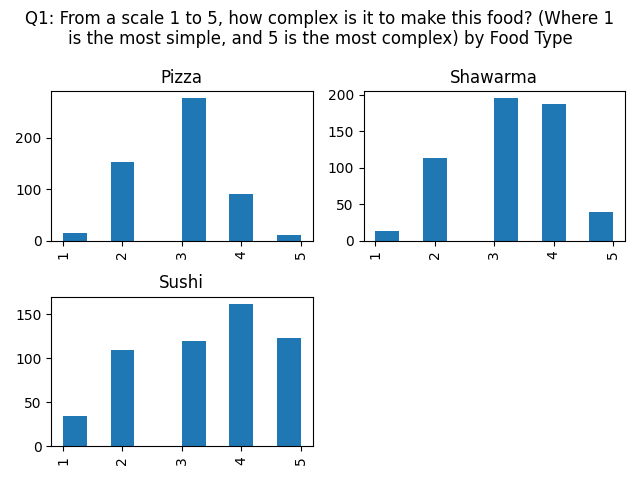
\includegraphics[width=\columnwidth]{data/histogram_Q1}}
    \caption{Input Size vs. Simulation Time for Nearest Neighbors and Comparison Sort for Different Regions on an X86MinorCPU.}
    \label{f:instruction_time}
\end{figure}

\begin{figure}[t!]
    \centerline{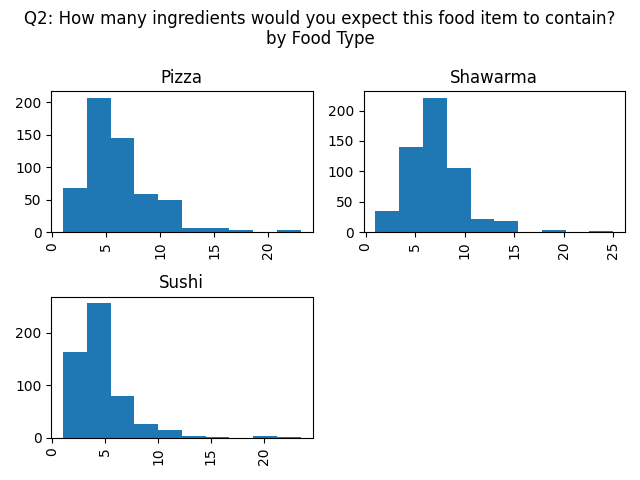
\includegraphics[width=\columnwidth]{data/histogram_Q2.png}}
    \caption{Input Size vs. Simulation Time for Nearest Neighbors and Comparison Sort for Different Regions on an X86MinorCPU.}
    \label{f:instruction_time}
\end{figure}

\begin{figure}[t!]
    \centerline{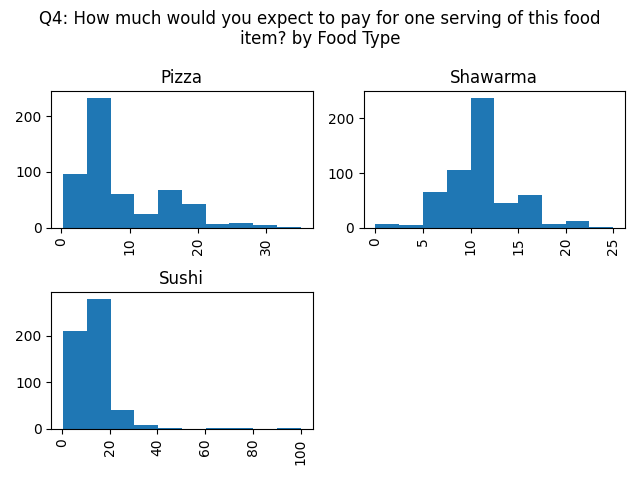
\includegraphics[width=\columnwidth]{data/histogram_Q4.png}}
    \caption{Input Size vs. Simulation Time for Nearest Neighbors and Comparison Sort for Different Regions on an X86MinorCPU.}
    \label{f:instruction_time}
\end{figure}